% =================================================================================
% Hier ausw�hlen, ob TUD-Design oder nicht
% =================================================================================
\newif\ifTUDdesign
\TUDdesigntrue					% TUD-Design
%\TUDdesignfalse				% F�r Rechner ohne installierte TUDdesign-Pakete
% =================================================================================


% =================================================================================
% Hier Daten f�r studentische Arbeit eingeben
% =================================================================================
\newcommand{\SADATyp}{Praktikumsbericht}
\newcommand{\SADATitel}{Versuch VI: Trajektorienfolgeregelung}
\newcommand{\SADAStadt}{Darmstadt}
\newcommand{\SADAAutor}{Andreas Jentsch, Ali Kerem Sacakli}
\newcommand{\SADABetreuer}{}
\newcommand{\SADABetreuerII}{}
\newcommand{\SADABetreuerIII}{}
\newcommand{\SADABegin}{}
\newcommand{\SADAAbgabe}{Praktikum Matlab/Simulink II \newline 11. Juli 2017}
\newcommand{\SADASeminar}{}
% =================================================================================


% =================================================================================
% Auswahl des IAT-Fachgebiets (rtm / rtp)
% =================================================================================
\newif\ifrtm
\rtmtrue	% rtm
%\rtmfalse	% rtp
% =================================================================================


% =================================================================================
% Erkl�rung, dass die Arbeit ohne Hilfe Dritter etc. erstellt wurde
% =================================================================================
\def\SADAVarianteErklaerung{ETIT}		% FB 18, Elektrotechnik
%\def\SADAVarianteErklaerung{MBDA}		% FB 16, Maschinenbau, Diplomarbeit
%\def\SADAVarianteErklaerung{MBSA}		% FB 16, Maschinenbau, Studienarbeit
% =================================================================================


% =================================================================================
% Ausnahmen von der automatischen Silbentrennung
% =================================================================================
\hyphenation{Aktu-ali-sie-rung Screen-shots Pa-rallel-ro-bo-ter Zu-stands-raum-mo-del-le nach-voll-zieh-bar Pro-jekt-se-mi-nar}
% =================================================================================


% =================================================================================
% Hier NIICHTS �ndern!
% =================================================================================
\ifTUDdesign
	\documentclass[11pt, twoside, colorback, accentcolor=tud2c, nopartpage, bigchapter, fleqn, ngerman, longdoc]{tudreport}
\else
	\documentclass[11pt, a4paper, twoside, fleqn, ngerman]{scrreprt}
  % F�r Entwurf auf Rechnern ohne installierte TUDdesign-Pakete	
	\usepackage{exscale}	% Korrektur math-Zeichen
	\usepackage{eurosym}
\fi
%To Do Package
\usepackage{todonotes}
%eps-plot von Matlab in pdf umwandeln, um diese einbinden zu k�nnen
\usepackage{epstopdf}
%Paket listings f�r das Einbinden von Quelltext
\usepackage{listings}
%Stil Matlab_colored definieren
\lstdefinestyle{Matlab_colored}
{
	language = Matlab,
	tabsize = 4,
	framesep = 3mm,
	frame = tb,
	classoffset = 0,
	basicstyle = \ttfamily,
	keywordstyle = \bfseries\color[rgb]{0,0,1},
	commentstyle = \itshape\color[rgb]{0.133,0.545,0.133},
	stringstyle = \color[rgb]{0.672,0.126,0.941},
	extendedchars = true,
	breaklines = true,
	prebreak = \textrightarrow,
	postbreak = \textleftarrow,
	numbers = left,
	numberstyle = \tiny,
	stepnumber = 5
}


\input{common/includes.tex}				% verwendete Pakete einbinden
\input{common/setup.tex}					% LaTeX-Einstellungen
\input{common/commonmacros.tex}		% oft verwendete Befehle
% =================================================================================


% =================================================================================
% Hier beginnt das eigentliche Dokument
% =================================================================================

\begin{document}
%\input{common/preface.tex} % Titelseite, Aufgabenstellung, Erkl�rung, Abstract, Inhaltsverzeichnis, etc.
\maketitle

\setcounter{chapter}{6}
%\setcounter{section}{7}
\section{Linearisierung}

Erg�nzend zum letzten Versuch, soll in diesem Versuch eine Trajektorienfolgeregelung entworfen werden. Hierbei soll nach Linearisierung der Trajektorie und Berechnung des Reglerparameters die Regelung in Simulink modelliert und anschlie�end simuliert werden. 

Folgendes Listing zeigt die Funktion zur Linearisierung der Trajektorie:

\lstinputlisting[style=Matlab_colored,caption={Quellcode der Funktion \textbf{linearisierung}}, label={linearisierung_XU}]{Codes/linearisierung_XU.m}


\section{Berechnen von K(t)}

Folgender Code implementiert die Riccati-DGL.

\lstinputlisting[style=Matlab_colored,caption={Quellcode der Funktion \textbf{RiccatiDGL}}, label={RiccatiDGL}]{Codes/RiccatiDGL.m}

Folgender Code dient zur Berechnung des Reglerparameters $\mathrm{K}(t)$.


\lstinputlisting[style=Matlab_colored,caption={Quellcode der Funktion \textbf{berechneK}}, label={berechneK}]{Codes/berechneK.m}

\newpage
\section{Folgeregelung unter Simulink}

Die Trajektorienfolgeregelung wird unter Ausnutzung der get�tigten Berechnungen in Simulink implementiert. Das folgende Bild zeigt das gesamte Simulink-Modell.
		\begin{figure}[htbp]
			\centering
			\includegraphics[width = 0.85\textwidth]{Bilder/Simulink.JPG}
			\caption{Modell der gesamten Trajektorienfolgeregelung}
			\label{fig:simulink}
		\end{figure}

\newpage
Um den Unterschied zwischen der reinen Steuerung und der Trajektorienfolgeregelung aufzuzeigen, werden im Nachfolgenden Plots gezeigt, wobei im zweiten und dritten Plot Parameter�nderungen durchgenommen worden sind.

		\begin{figure}[htbp]
			\centering
			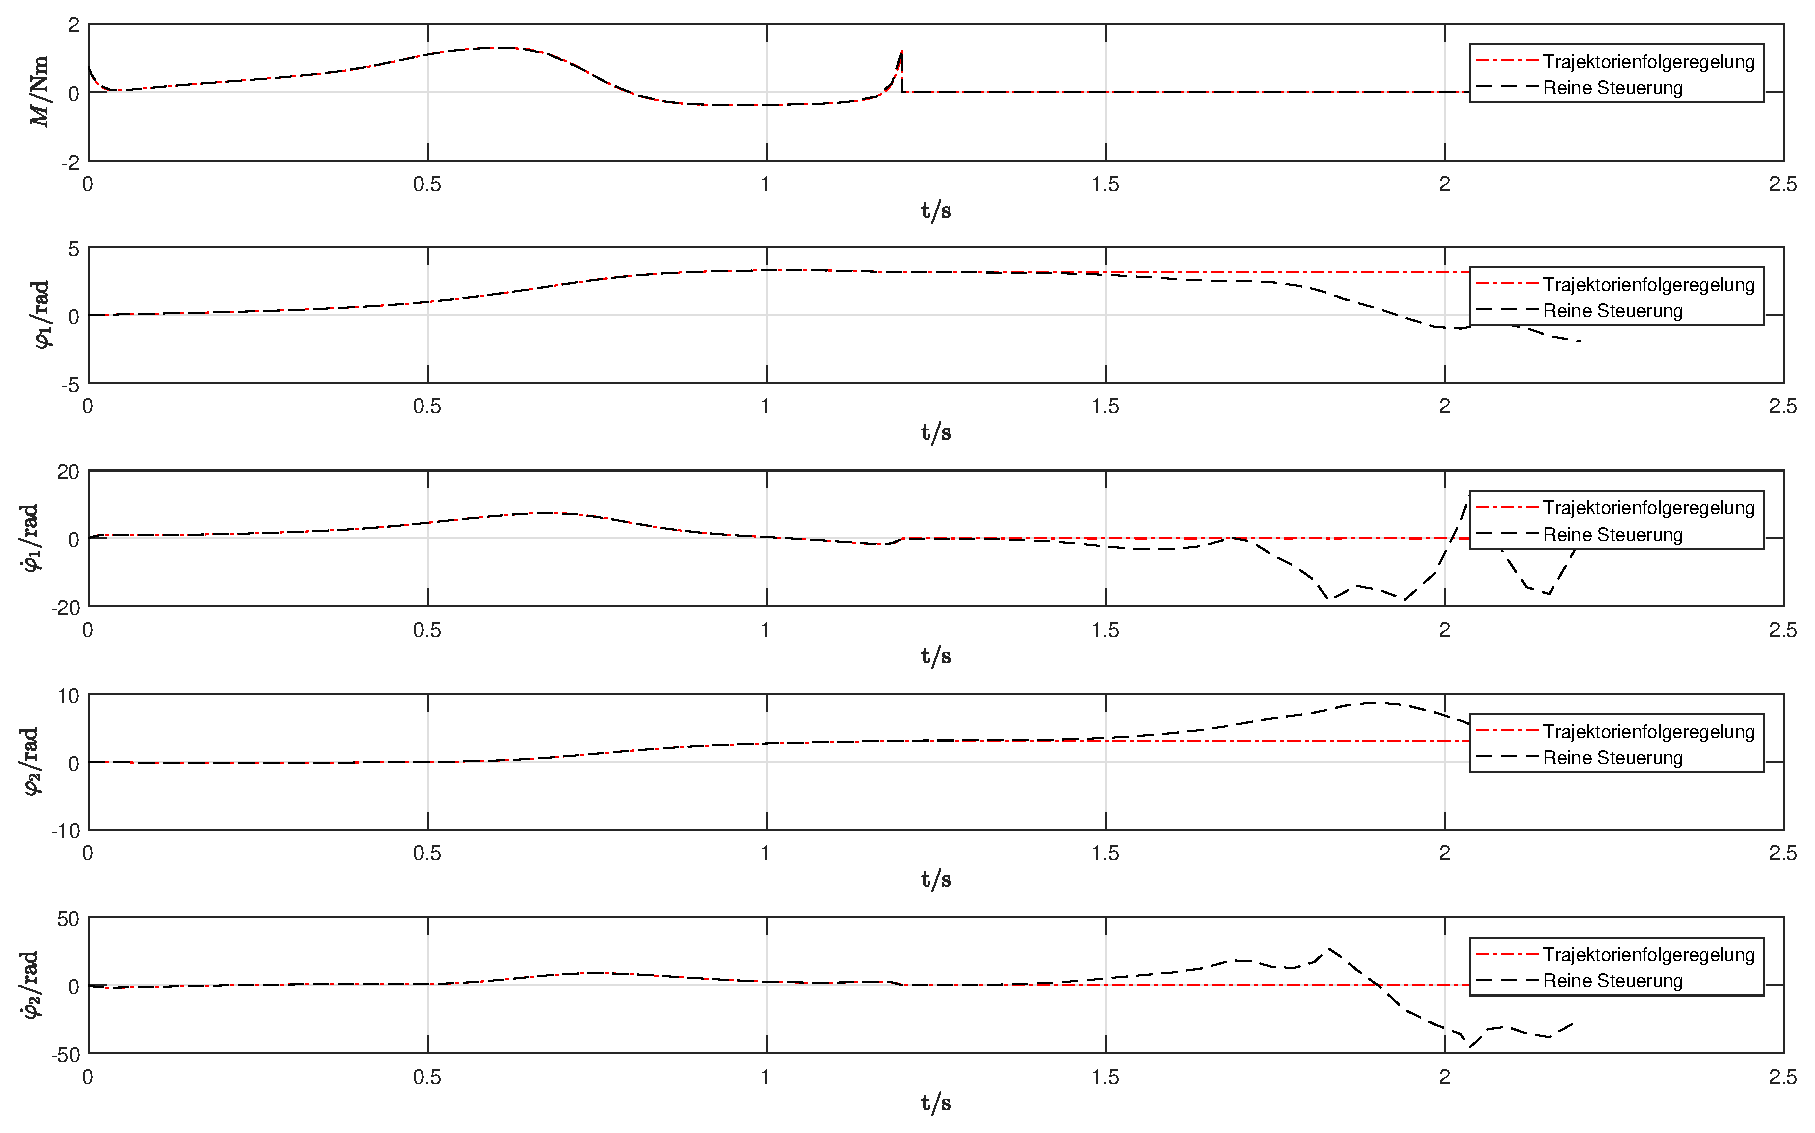
\includegraphics[width = \textwidth]{Bilder/Sim_ohneParameteraenderung.eps}
			\caption{Plot der Zust�nde ohne Parameter�nderung}
			\label{fig:sim1}
		\end{figure}
		
		\begin{figure}[htbp]
			\centering
			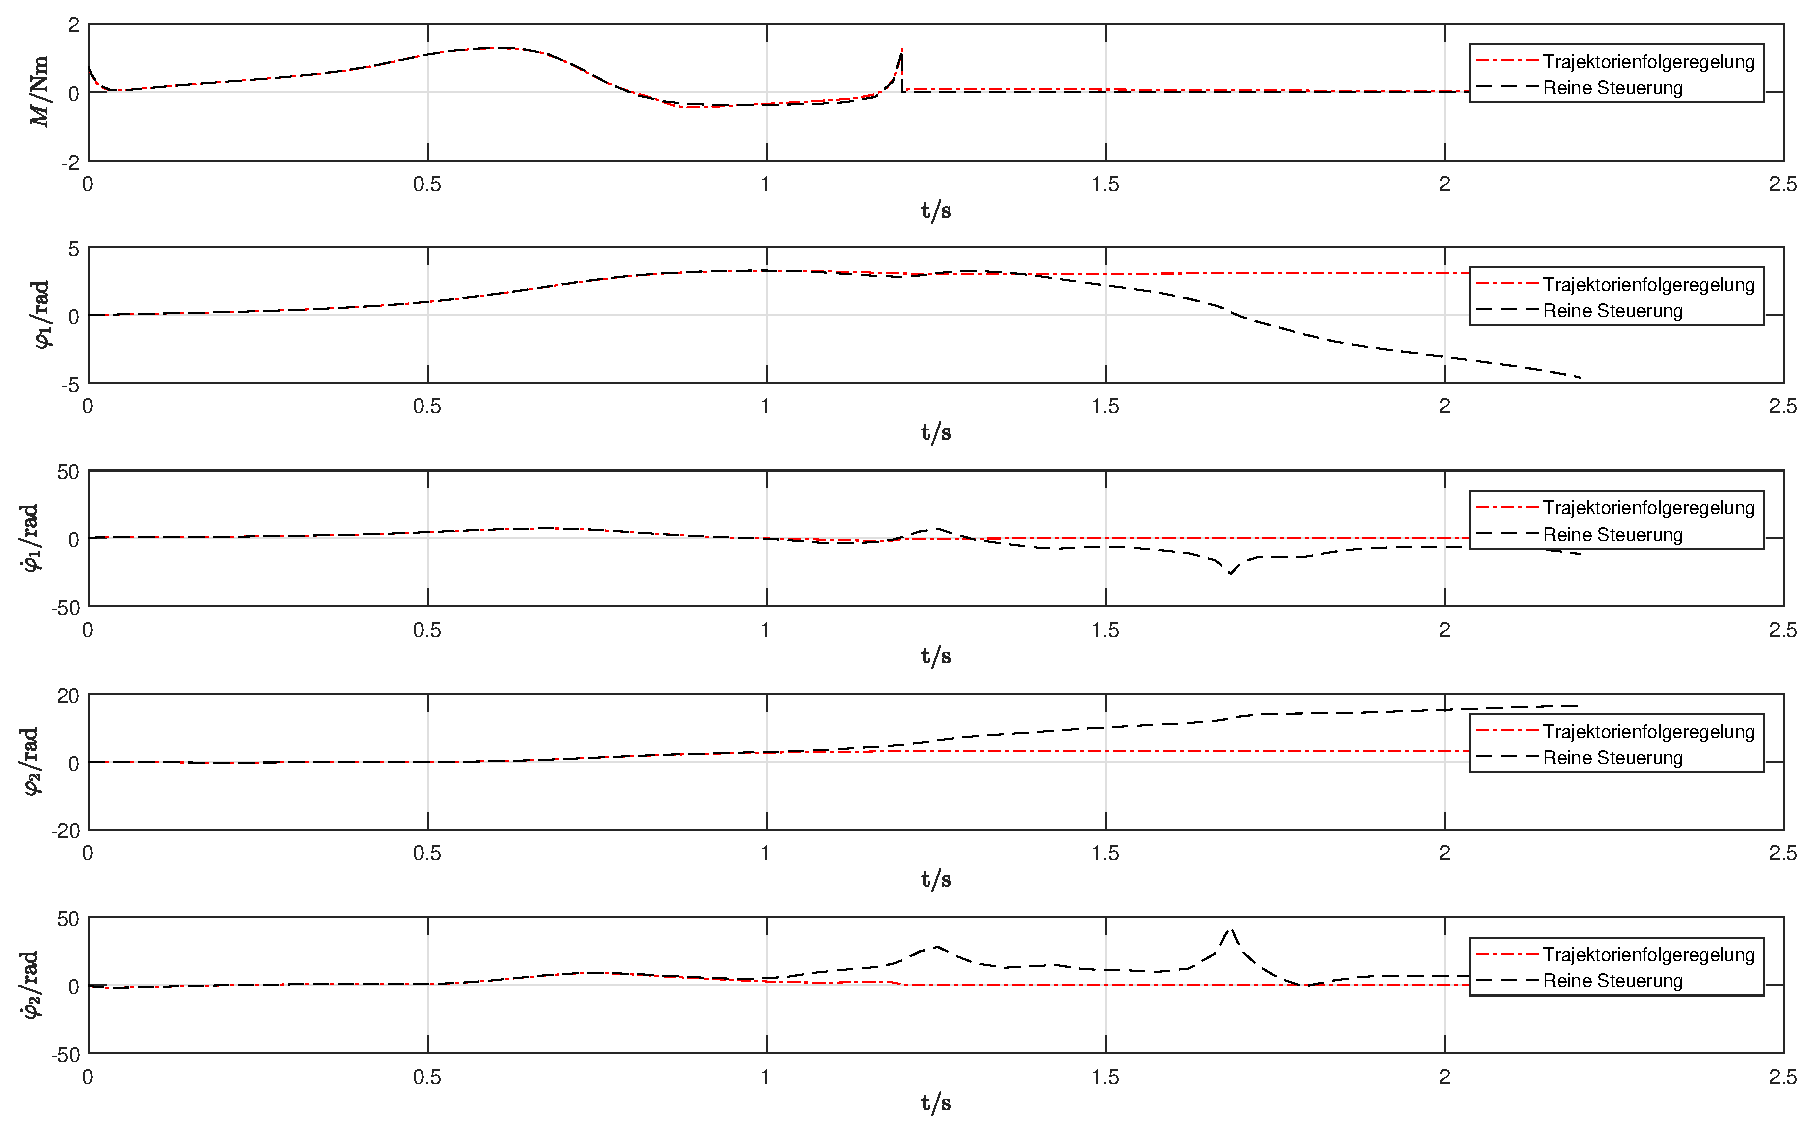
\includegraphics[width = \textwidth]{Bilder/Sim_kuerzeresZweitesPendel.eps}
			\caption{Plot der Zust�nde mit 5\% k�rzerem zweiten Pendel}
			\label{fig:sim2}
		\end{figure}
						
		\begin{figure}[htbp]
			\centering
			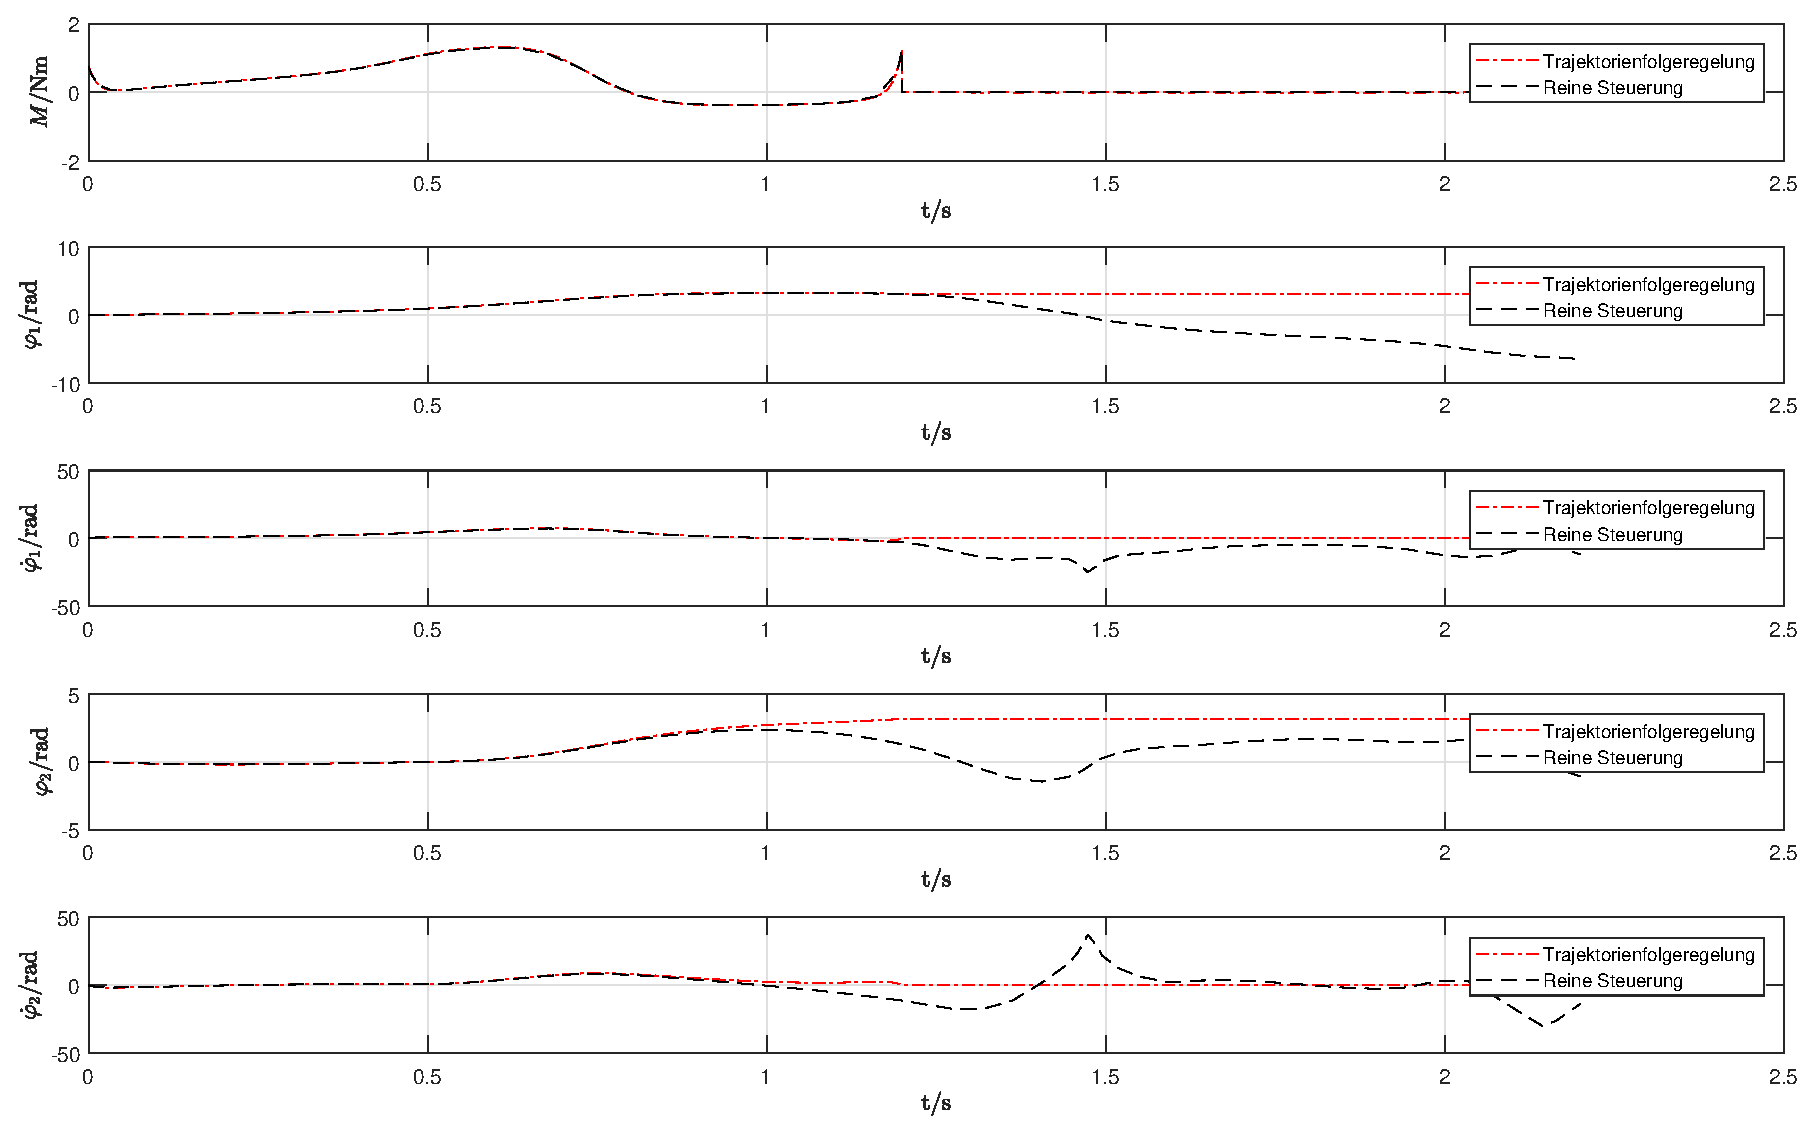
\includegraphics[width = \textwidth]{Bilder/Sim_schwereresErstesPendel.eps}
			\caption{Plot der Zust�nde mit schwererem ersten Pendel}
			\label{fig:sim3}
		\end{figure}

\newpage
		
\todo[inline]{Welche Unterschiede stellen Sie beim Vergleich de reinen Steuerung und der Steuerung mit Folgeregelung fest?}

\begin{itemize}
	\item Ohne Parameter�nderung: bis Ende der �bergangszeit stimmen Steuerung und Regelung �bereinander. Danach ist Steuerung instabil, jedoch Regelung stabil (station�r genau)
	\item mit Paramet�nderungen: Unterschiede sind schon w�hrend der �bergangszeit (besonders gegen Ende der �bergangszeit) zu sehen. Nach der �bergangszeit so wie ohne Parameter�nderung (Steuerung instabil, Regelung stabil, station�r genau)
\end{itemize}

\section{Einfluss des Antriebs}

\todo[inline]{Motor modellieren}
\todo[inline]{Vergleichen mit System vorher, verschiedene Tm ausprobieren--> Wertebereich von Tm bestimmen}


\end{document}
